\documentclass[a4paper,12pt]{article}
\usepackage{graphicx}
\graphicspath{{.}}

\usepackage{calc}
\setlength\textwidth{7in}
\setlength\textheight{10in}
\setlength\oddsidemargin{(\paperwidth-\textwidth)/2 - 1in}
\setlength\topmargin{(\paperheight-\textheight
	-\headheight-\headsep-\footskip)/2 - 1in}

\begin{document}

	
	\title{Tema Curs 6 Baze de Date}
	\author{Moroianu Theodor (135)}
	\date{\today}
	\maketitle

	\section{Diagrama Relationala\newline}
	
		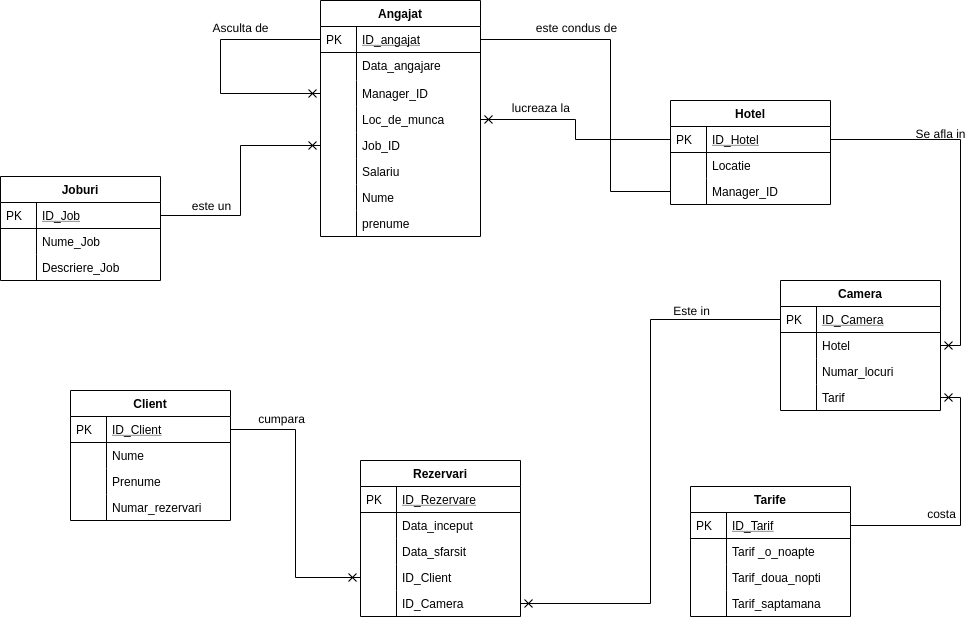
\includegraphics[scale=0.52]{diagrama_tema_6_curs.png}
		
		\newpage
	
	\section{Scheme Relationale}
	
		\begin{itemize}
			\item \textbf{Angajat:} \underline{ID\_ANGAJAT}, Data\_angajare, Manager\_ID, Loc\_de\_munca, Job\_ID, Salariu, Nume, Prenume 
			\item \textbf{Client:} \underline{ID\_Client}, Nume, Prenume, Numar\_rezervari
			\item \textbf{Joburi:} \underline{ID\_Job}, Nume\_Job, Descriere\_Job
			\item \textbf{Rezervari:} \underline{ID\_Rezervare}, Data\_inceput, Data\_sfarsit, ID\_Client, ID\_Camera
			\item \textbf{Camera:} \underline{ID\_Camera}, Hotel, Numar\_locuri, Tarif
			\item \textbf{Tarife:} \underline{ID\_Tarif}, Tarif\_o\_noapte, Tarif\_doua\_nopti, Tarif\_saptamana
			\item \textbf{Hotel:} \underline{ID\_Hotel}, Locatie, Manager\_ID
		\end{itemize}
	
	\section{Extemple de operatii algebrice relationale}
	
	\subsection{Sa se afiseze numele tututor clientilor ai hotelului}
		
		\begin{itemize}
			\item \textbf{SQL:\\}
			\textit{SELECT nume, prenume\\
			FROM client;}
		
			\item \textbf{Algebra Relationala:\\}
			\textit{PROJECT(client, nume, prenume)}
		\end{itemize}	
			
		
	\subsection{Sa afiseze toti clientii care au facut cel putin o rezervare}
		
		\begin{itemize}
			\item \textbf{SQL:\\}
			\textit{SELECT DISTINCT nume, prenume\\
				FROM client c, rezervari r\\
				WHERE c.ID\_Client = c.ID\_Client;}
			
			\item \textbf{Algebra Relationala:\\}
			\textit{c = SEMIJOIN(client, rezervari, client.id\_client = rezervari.id\_client)\\
				answer = PROJECT(c, nume, prenume)}
		\end{itemize}	
		
		\subsection{Sa afiseze toti clientii si angajatii}
		
		\begin{itemize}
			\item \textbf{SQL:\\}
			\textit{SELECT nume, prenume, 'Angajat'\\
				FROM angajat\\
				UNION\\
				SELECT nume, prenume, 'Client'\\
				FROM client;}
			
			\item \textbf{Algebra Relationala:\\}
			\textit{c = PRODUCT(PROJECT(clienti, nume, prenume), "client")\\
				a = PRODUCT(PROJECT(angajati, nume, prenume), "angajat")\\
				answer = UNION(c, a)}
		\end{itemize}	
		
	
	\subsection{Sa se afiseze toate rezervarile de o noapte la o camera care costa intre 300 si 400 pe noapte}
	
		\begin{itemize}
			\item \textbf{SQL:\\}
			\textit{SELECT id\_rezervare\\
				FROM rezervari r, camera c\\
				WHERE r.id\_camera = c.id\_camera\\
				        AND (SELECT tarif\_o\_noapte\\
				 	    FROM tarife\\
				 	    WHERE id\_tarif = c.tarif) BETWEEN 300 AND 400);}
			
			\item \textbf{Algebra Relationala:\\}
			\textit{t = SELECT(tarife, $\leq$ 300 tarif\_o\_noapte $\leq$ 400)\\
				c = SEMIJOIN(camera, t)\\
				answer = SEMIJOIN(rezervari, c)}
		\end{itemize}	
	
	
	\subsection{Sa se afiseze managarul hotelului la care lucreaza angajatul cu ID 400}
	
	\begin{itemize}
		\item \textbf{SQL:\\}
		\textit{SELECT m.nume, m.prenume\\
			FROM angajat m, hotel h, angajat p\\
			WHERE p.id\_angajat = 400\\
			AND p.loc\_de\_munca = h.id\_hotel\\
			AND h.manager\_id = m.id\_angajat;}
		
		\item \textbf{Algebra Relationala:\\}
		\textit{h = PROJECT(SELECT(angajat, id\_angajat = 400), loc\_de\_munca)\\
			m = PROJECT(SELECT(hotel, id\_hotel = h), manager\_id)\\
			answer = PROJECT(SELECT(angajat, id\_angajat = m), nume, prenume)}
	\end{itemize}	
	
	
\end{document}















